\documentclass[11pt]{article}
\usepackage[margin=1in]{geometry}
\usepackage{booktabs}
\usepackage{graphicx}
\usepackage{amsmath}
\usepackage{microtype}
\usepackage[hidelinks]{hyperref}
\usepackage{xspace}

\newcommand{\us}{\,\textmu s\xspace}

\title{Bounded Tile-Level Preemption in Persistent Kernels Without Hopper:\\
A Measurement Study on Ampere}
\author{Ayaan Faisal\\ Rutgers University\\ \texttt{af1174@scarletmail.rutgers.edu}}
\date{August 2026}

\begin{document}
\maketitle

\begin{abstract}
ExpertPlex preempts work inside a persistent GPU kernel at tile
granularity, with a bound of one tile time plus one check epoch, and
attributes both the bound and the safety of the mechanism to three
Hopper (sm\_90) primitives: thread-block clusters, distributed shared
memory, and TMA multicast. We measure what remains of the mechanism on
hardware that has none of them. On an NVIDIA A10 (sm\_86), with claims
and thresholds registered before any measurement code was written,
per-block independent polling of a single global flag preempts a
saturated persistent kernel in 59\us{} median (70.7\us{} p99) at 0.8\%
steady-state overhead, against a no-preemption baseline of 957\us.
Across a 24-cell sweep of resident blocks ($16{-}288$) and poll period
($1{-}8$), flag propagation stays at 1--3\us{} at every block count;
latency growth is entirely tile-time growth under SM co-residency.
Checking the flag inside a \texttt{cp.async}-pipelined tile lowers the
bound to 18.4\us{} median (23.6\us{} p99) at 5.0\% overhead, inside the
2.2--25.3\us{} tile-boundary band ExpertPlex reports on 8$\times$H800.
Safety: across 10,000 forced mid-pipeline yields that reuse shared
memory with a copy group outstanding, a one-instruction drain
discipline produced zero corrupt outputs against a float64 reference
(95\% upper bound $3.7\times10^{-4}$); a planted-fault control
confirmed the detector. The one dangerous failure we encountered was
control divergence in the check protocol, not a data race: a single
omitted barrier corrupted whole tiles in roughly half of runs.
\end{abstract}

\section{Introduction}

A persistent kernel sizes its grid to the hardware rather than the
problem: blocks never exit, and pull work from an in-memory queue.
Megakernel systems compile entire model forward passes into one such
kernel and remove every kernel boundary a conventional scheduler could
preempt at~\cite{mpk}. A separate line of work manufactures preemption
points the megakernel line removes~\cite{lithos,hummingbird}.
ExpertPlex~\cite{expertplex} bridges the two: an adaptive persistent
kernel that preempts prefill for decode at tile granularity, bounded by
one tile execution plus one check epoch. Its mechanism is built on
sm\_90 primitives, and it states the design constraint directly:
``independent tile-boundary checks are unsafe because high-performance
operations pipeline both warps and CTAs across tiles.''

Every GPU below sm\_90 lacks the primitives that statement leans on.
Whether bounded tile-level preemption is therefore unavailable below
Hopper, or merely unmeasured, is an empirical question. This paper
measures it.

We registered a claim and its falsifier before writing measurement
code (Section~\ref{sec:claims}), built the mechanism in its simplest
form---one global flag, polled independently by every block---and
measured three things on an NVIDIA A10: what preemption costs, how the
cost and latency scale with resident blocks and poll period, and
whether the mechanism is safe when a yield lands mid-pipeline.

Contributions, each a measurement:
\begin{enumerate}
\item \textbf{A baseline.} With every residency slot occupied, an
  urgent task waits for the full remaining drain: 957\us{} median,
  correlation $0.9934$ with remaining queue length. Stream priority
  does not help; priorities order pending blocks and cannot evict
  resident ones. One free slot collapses the wait to 76\us{}
  (Section~\ref{sec:baseline}).
\item \textbf{The two numbers.} Independent per-block polling costs
  0.8\% steady-state at full occupancy (worst case across code
  variants: 3.4\%, against a pre-registered 10\% falsifier) and
  preempts in 59.4\us{} median / 70.7\us{} p99 over 10,000
  device-timestamped events (Section~\ref{sec:boundary}).
\item \textbf{The scaling surface.} Over resident blocks
  $\{16,36,72,144,216,288\}$ $\times$ poll period $\{1,2,4,8\}$, the
  check epoch never exceeds 3\us{} and does not grow with block count.
  Latency grows $8.4\times$ to saturation entirely through tile-time
  stretch under SM co-residency. The registered alternative
  hypothesis---that propagation dominates without cluster
  primitives---fails both of its tests (Section~\ref{sec:surface}).
\item \textbf{A safety result with a negative control.} 10,000 forced
  yields inside a \texttt{cp.async} pipeline, each reusing shared
  memory that an uncommitted copy group targets, produced zero corrupt
  outputs under a drain discipline; a poison control was caught
  10,000/10,000 times. Checking inside the pipeline lowers preemption
  to 18.4\us{} median at 5.0\% overhead---inside ExpertPlex's reported
  Hopper band (Section~\ref{sec:safety}).
\item \textbf{A relocated hazard.} The failure that actually produced
  silent corruption was not a data race but control divergence: an
  omitted barrier in the check protocol let warps of one block resolve
  the yield branch differently, and sm\_70+ barrier semantics let the
  divergent halves run permanently phase-shifted
  (Section~\ref{sec:hazard}).
\end{enumerate}

The study is a characterization, not a system: one GPU model, one
kernel shape, synthetic tiles. Section~\ref{sec:threats} states the
limits. Code, raw distributions, and the run log are
public.\footnote{\url{https://github.com/AyaanFaisal21/APK}}

\section{Background}

\paragraph{The mechanism under test.} ExpertPlex schedules at
CTA-cluster granularity because ``CTAs connected by TMA multicast must
execute the same tile''; one CTA per cluster checks the preemption flag
at a tile boundary and propagates the decision through distributed
shared memory. Measured tile boundaries arrive every 2.2--25.3\us,
independent of operation length, so preemption is bounded by one tile
plus one cluster-local check epoch~\cite{expertplex}. Below sm\_90
there are no clusters, no DSMEM, and no TMA: flag propagation must
cross L2, and no hardware couples the fates of neighboring CTAs.

That absence cuts both ways, and the two directions are the two halves
of this study. Propagation through L2 rather than shared memory could
make the check epoch dominant (the cost question). The absence of
cross-CTA coupling could make independent checks safe by construction
(the safety question): the pipelining ExpertPlex's warning describes is
precisely the coupling sm\_86 cannot express between blocks, leaving
only the intra-block half of the hazard---\texttt{cp.async} copies in
flight into shared memory.

\paragraph{Lineage.} In-kernel yield predates Hopper: Cooperative
Kernels~\cite{coopkernels} had persistent workgroups surrender
resources on OpenCL~2.0 hardware in 2017. Hopper made the primitive
cheap; it did not invent it. That lineage is why we treat
``unavailable below Hopper'' as a hypothesis rather than a fact.

\section{Registered claims}
\label{sec:claims}

The claim file was committed before any measurement code and never
edited; its git history is the audit trail. Verbatim thresholds:

\textbf{N1.} Bounded tile-level preemption works on Ampere without
cluster primitives at cost comparable to Hopper, because the bound is
dominated by tile execution (2.2--25.3\us{} per ExpertPlex) and the
check-propagation epoch is negligible.

\textbf{A-N1 (falsifier).} Preemption on Ampere is propagation-bound:
the check epoch is comparable to or larger than tile time, and degrades
with resident block count.

\textbf{Thresholds, fixed in advance.} Cost is comparable if
steady-state overhead with polling enabled is ${\le}10\%$ (ExpertPlex
reports ${\sim}8\%$ decode overhead). The mechanism is
propagation-bound if the check epoch exceeds 25\% of median tile time
or grows more than $2\times$ from 16 to 72 resident blocks. Latency is
measured on-device; every quoted p99 requires ${\ge}10{,}000$ events;
correctness after any yield is checked against a float64 reference,
never against another run of the same kernel; tile durations are held
in the 2--25\us{} band.

\section{Method}
\label{sec:method}

\paragraph{Workload.} The unit of work is one $64\times64$ SGEMM tile
computed cooperatively by a 256-thread block, with inner dimension $K$
as the duration knob: $K\in\{32,64,128\}$ gives 6.7, 10.3, 17.8\us{}
median at one block per SM (all measurements use $K=64$ unless
stated). A persistent kernel pulls tiles from a global queue by atomic
fetch-add. Tasks cycle a fixed tile grid, so repeated writes are
idempotent and the output remains verifiable at any task count.

\paragraph{Definitions.} \emph{Preemption latency} is the interval
from the flag-set instant to the last resident block reaching a yield
point (a boundary at which it could switch work). \emph{Check epoch}
is the interval from set to the first observation---the propagation
plus polling-alignment term the registered falsifier is about.
\emph{Overhead} is the drain-time ratio of the polling kernel to an
identical kernel with the poll compiled out, no events fired.

\paragraph{Timestamping.} All cross-block intervals use
\texttt{\%globaltimer}, which we measured to tick in 1.024\us{}
quanta on GA102; epoch readings therefore sit at instrument
resolution and are reported as bounds. The set instant is produced two
independent ways: \emph{device-set} (block~0 writes the flag at
pre-scheduled instants and logs the timer at the write; no clock-domain
crossing; the primary instrument) and \emph{host-set} (the host writes
the flag; its clock is mapped onto the device timer by a spin-kernel
calibration). The two agree within 0.6\us{} after correcting a
${\sim}10$\us{} bias in the idle-measured calibration---itself a
finding: idle-link calibrations do not transfer to loaded runs.
Because block~0's own next check is phase-locked one tile behind its
write, the analysis reports latency with and without the setter block;
at ${\ge}144$ blocks the setter is never the last observer.

\paragraph{Verification.} Every configuration is gated before
measurement: outputs checked element-wise against a float64 host
reference at $\mathrm{atol}=\mathrm{rtol}=10^{-4}$; output buffers
NaN-filled before every run so unexecuted work fails loudly;
\texttt{compute-sanitizer} clean after every kernel change. The safety
experiment adds a planted-fault control (Section~\ref{sec:safety}):
a zero-corruption result is accepted only alongside proof the detector
fires.

\paragraph{Environment.} NVIDIA A10 (GA102, sm\_86, 72 SMs, 24\,GB),
driver 580.105.08, CUDA 12.8. SM clock locked at 1200\,MHz and read
back \emph{under load}: the 150\,W power limit---which equals the
card's maximum---throttles through nominally accepted locks at 1695 and
1350\,MHz. Occupancy is pinned to 4 blocks/SM at compile time after a
register-allocation change silently reduced it and orphaned 72 of 288
blocks; grids exceeding residency are refused. Warmup iterations and
the first 100 events of every run are discarded. Primary results were
reproduced on a second physical A10 within 2\% (the tile median within
1.6\%, the float64 error bit-identical).

\paragraph{Exclusions, with cause.} Two measurement cells are reported
but not interpreted. At exactly 72 blocks (one per SM) block placement
is bistable---drain times are bimodal, 12\% apart, sticky per launch
sequence---so A/B overhead comparison there is meaningless. The poll
period axis of the \emph{overhead} surface is confounded by code
generation: the period-1 template variant spills 8 bytes per tile
where the others spill 16, a difference larger than the polling effect;
only period-1 columns are compared across builds. The cost verdict
quotes the worst case over all variants and cells.

\section{Results}

\subsection{Baseline: no preemption}
\label{sec:baseline}

With all 288 residency slots occupied by the persistent kernel, an
urgent single-tile kernel launched on a maximum-priority stream waits
957\us{} median, 1476\us{} p99 ($n{=}2000$). The wait is the remaining
drain: correlation with remaining queue length at arrival is $0.9934$,
slope 88.1\,ns/task $\times$ 288 workers $=$ 25.4\us{} per tile,
matching the independently measured co-resident tile time. Priority
never helps; it orders pending blocks and cannot evict resident ones.
Residency shape, not utilization, is the operative condition: with one
slot left open the same urgent tile completes in 76\us, and with 72
blocks on 72 SMs, in 26\us. A baseline measured at the wrong residency
shape would be optimistic by up to $37\times$.

\subsection{The yield at tile boundaries}
\label{sec:boundary}

The mechanism is one flag in device memory; each block issues one
volatile read per tile boundary and acts on it independently.

\textbf{Cost.} Polling every boundary costs 0.80\% of drain throughput
at full occupancy (median of 20 interleaved A/B drains). The worst
overhead measured in any valid cell of any code variant is 3.4\%. The
registered falsifier is 10\%. N1 holds on the cost axis.

\textbf{Latency.} Over 10,000 device-set events: 59.4\us{} median,
70.7\us{} p99. The first observer reacts in 1.0\us{} median; the
remainder is waiting for the slowest in-flight tile. This is the
finding that revises the bound's denomination: under 4-way
co-residency, individual tile walls spread from a 25.4\us{} throughput
mean to a 57.6\us{} p99 (measured directly), and the preemption
latency distribution sits on the max of ${\sim}288$ in-flight
residuals---even the fastest of 10,000 events took 51\us. The ``one
tile execution'' term in the ExpertPlex bound is, on a saturated
Ampere part, the \emph{contention-stretched worst-case} tile, at this
geometry $2.3\times$ the mean. The urgent task itself completes far
sooner: 21\us{} median on device-timeline endpoints (${\sim}30\times$
over baseline with endpoint-matched accounting), because the first
observer claims the work while stragglers finish their tiles.

\subsection{The scaling surface}
\label{sec:surface}

\begin{figure}[t]
  \centering
  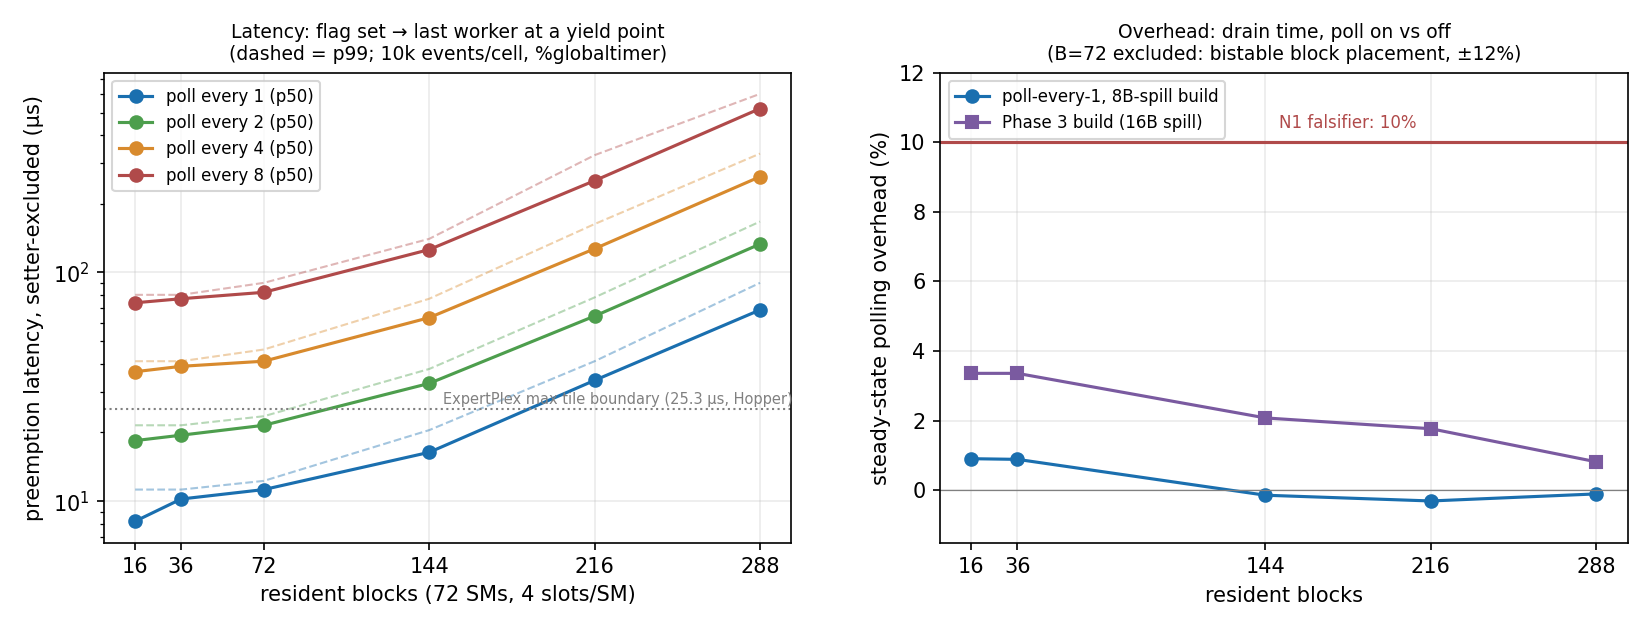
\includegraphics[width=\linewidth]{figures/phase4_surface.png}
  \caption{Left: preemption latency (setter-excluded p50, dashed p99)
  versus resident blocks for four poll periods; the horizontal rule is
  ExpertPlex's reported maximum tile boundary interval on Hopper.
  Right: steady-state overhead versus the registered 10\% falsifier;
  the 72-block cell is excluded (bistable placement). 10,000 events
  per cell, zero anomalies.}
  \label{fig:surface}
\end{figure}

\begin{table}[t]
  \centering
  \caption{Latency at poll period 1 (setter-excluded, \us). The check
  epoch (first-observation delay) never exceeds three timer quanta and
  does not grow with block count; latency growth is tile-time growth
  under SM co-residency.}
  \label{tab:surface}
  \begin{tabular}{rrrrr}
    \toprule
    blocks & p50 & p99 & epoch p50 & overhead \\
    \midrule
    16  & 8.2  & 12.3 & 3.1 & 0.9\% \\
    36  & 10.2 & 11.3 & 1.0 & 0.9\% \\
    72  & 11.3 & 13.3 & 1.0 & --- \\
    144 & 16.4 & 20.5 & 1.0 & $\approx$0 \\
    216 & 33.8 & 41.0 & 1.0 & $\approx$0 \\
    288 & 68.6 & 90.1 & 2.0 & $\approx$0 \\
    \bottomrule
  \end{tabular}
\end{table}

Table~\ref{tab:surface} and Figure~\ref{fig:surface} give the surface.
Three facts decide the registered verdict. The epoch stays at 1--3\us{}
(1--3 timer quanta) at every block count and \emph{shrinks} from 16 to
72 blocks, where A-N1 requires more than $2\times$ growth. The epoch
never approaches 25\% of median tile time except in the 16-block cell,
where the $3.1/10.2$ reading is set by timer resolution and poller
sparsity, not propagation---reported as a threshold crossing with
cause. And latency at fixed poll period scales $1.94$--$2.25\times$
per doubling of poll period at every block count, exactly as a
residual-wait model predicts. A-N1 fails; N1 holds; the latency that
does grow ($8.4\times$ from 16 to 288 blocks) is contention physics,
which no cluster primitive would remove. The saturation-point median
varies 54--69\us{} across code variants of the same mechanism (tile
walls shift with register allocation), so we quote it as a range;
cells at ${\le}144$ blocks reproduce to the timer quantum across
builds.

\subsection{Mid-pipeline safety}
\label{sec:safety}

The boundary yield never interrupts a pipeline; ExpertPlex's warning is
about checks that do. We rebuilt the tile with the staging real kernels
use---\texttt{cp.async} copies, double-buffered, one commit group per
16-deep chunk---and forced the claiming block to yield at
stage boundaries \emph{while a copy group is outstanding} into the
shared memory the urgent tile is about to reuse. Three disciplines,
10,000 events each, every urgent output checked against float64:

\begin{table}[h]
  \centering
  \caption{Forced mid-pipeline yields reusing in-flight shared memory.}
  \label{tab:safety}
  \begin{tabular}{lrrl}
    \toprule
    discipline & corrupt & worst rel.\ err & background C \\
    \midrule
    drain (\texttt{wait\_all} first) & 0 / 10{,}000 & $1.4\times10^{-6}$ & pass \\
    naive (no wait)                  & 0 / 10{,}000 & $1.4\times10^{-6}$ & pass \\
    poison (planted fault)           & 10{,}000 / 10{,}000 & $9.9\times10^{-1}$ & pass \\
    \bottomrule
  \end{tabular}
\end{table}

The drain result is the claim: with one \texttt{cp.async.wait\_all}
before shared-memory reuse, zero corruption in 10,000 mid-pipeline
yields (95\% upper bound $3.7\times10^{-4}$ by the rule of three),
against a control that proves the detector fires on a single wrong
value. The naive zero is deliberately \emph{not} promoted to a claim:
at this geometry the outstanding group was issued a full stage-compute
(${\sim}5$\us) before the yield point and \texttt{cp.async} copies land
in well under a microsecond, so the bookkeeping outlives the physical
hazard; the pre-registered risk note anticipated exactly this reading,
and window-widening variants are future work.

Checking inside the pipeline is also the latency payoff: at full
saturation, stage-granularity polling yields 18.4\us{} median /
23.6\us{} p99 at 5.0\% overhead, versus 50.2\us{} / 58.4\us{} at 2.0\%
for boundary polling on the same tile. The mid-pipeline figure sits
inside the 2.2--25.3\us{} tile-boundary band ExpertPlex reports on
8$\times$H800. The study's latency arc is
$957 \rightarrow {\sim}66 \rightarrow 18.4$\us: baseline, boundary
yield, disciplined mid-pipeline yield.

\subsection{The hazard that did fire}
\label{sec:hazard}

The only silent corruption in five phases of measurement came from the
check protocol itself. An early revision compared live shared values
(\texttt{s\_flag} against \texttt{s\_lastSeen}) while thread~0 updated
the latter inside the branch; a late warp could read the updated value
and skip a branch its block had entered. On sm\_70+ barriers match by
arrival count, not program location, so the divergent halves both
released, and the block ran permanently phase-shifted---emitting
whole-tile garbage until kernel exit, in roughly half of runs, with
plausible magnitudes throughout. The instrument caught it (a poison
gate failing on the \emph{background} matrix it cannot reach), the fix
is a barrier-protected snapshot of shared state before the branch, and
21/21 post-fix runs are clean ($P<10^{-6}$ under the prior failure
rate). We report it as a result rather than an embarrassment because it
relocates the risk: in 10,000 tries the data race ExpertPlex's
cluster reasoning warns about never fired on this hardware, while the
control-divergence hazard in an independent-check protocol fired in
half of all runs. On Ampere, ``independent checks are hard'' is true,
but the difficulty lives in control flow, not data.

\section{Threats to validity}
\label{sec:threats}

One GPU model, one vendor, one node; claims about Hopper are cited,
not measured. One kernel shape and one tile size ($K{=}64$) on the
surface; the tile is synthetic (a real-model port is future work).
``Saturated'' is shape-specific: registers bind at 4 blocks/SM for
this kernel pair, and a smaller urgent kernel could co-schedule where
ours could not. The timer quantum (1.024\us) floors every epoch
reading. The naive-discipline zero is scoped to this pipeline
geometry. Overhead comparisons across poll periods are
codegen-confounded and excluded; the quoted worst case spans all
variants. Baseline and Phase-3/5 e2e figures use different endpoint
conventions; both are reported and the matched ratio
(${\sim}30\times$) is the conservative one.

\section{Related work}

ExpertPlex~\cite{expertplex} is the object of study; its mechanism,
bound, and safety claim are quoted throughout.
MPK~\cite{mpk} compiles inference into megakernels and reports a
bandwidth floor that makes megakernels a lever that largely finishes;
it does not preempt. LithOS~\cite{lithos} is the opposing thesis,
atomizing kernels to create the preemption points megakernels remove.
Hummingbird~\cite{hummingbird} reaches microsecond preemption on
closed-source GPUs under kernel-per-op execution. Cooperative
Kernels~\cite{coopkernels} established in-kernel yield on 2017
hardware. The megakernel and GPU-scheduling literatures are otherwise
nearly disjoint; this study measures the bridge on hardware the bridge
was not built for.

\section{Conclusion}

On a pre-registered protocol, bounded tile-level preemption
generalizes below Hopper. The check epoch that cluster primitives
accelerate is 1--3\us{} on Ampere and never dominant; the bound is
denominated in contention-stretched tile time, which clusters would
not change. With a one-instruction drain discipline, mid-pipeline
yields are safe in 10,000 of 10,000 float64-verified trials, and put
preemption latency inside the band ExpertPlex reports on Hopper---at
5\% overhead, on a \$3,000 part. The hazard that justifies
cluster-coordinated checking on Hopper did not manifest on sm\_86; the
hazard that did manifest is a barrier-discipline bug any independent
protocol must design against. For every Ampere GPU in the world, the
scheduler inside a persistent kernel is not waiting on hardware.

\section*{Artifact and disclosure}

Code, registered claims with git-provable timestamps, raw per-event
distributions, the figure pipeline, and a dated run log including all
eight faults found during the study are at
\url{https://github.com/AyaanFaisal21/APK}. AI tools (Claude) assisted
with code and documentation; the author directed, reviewed, and
verified all work. No measured number comes from a model: every result
is produced by the released instruments under the registered
thresholds, and primary results were reproduced on a second device.

\begin{thebibliography}{9}

\bibitem{expertplex}
Wu et al.
\newblock ExpertPlex: Fine-grained phase multiplexing for MoE serving
with adaptive persistent kernels.
\newblock arXiv:2607.18002, 2026.

\bibitem{mpk}
Mirage Persistent Kernel team.
\newblock MPK: Compiling multi-GPU inference into a single megakernel.
\newblock arXiv:2512.22219, OSDI 2026.

\bibitem{lithos}
Skarlatos et al.
\newblock LithOS: An operating system for GPU-accelerated datacenters.
\newblock arXiv:2504.15465, SOSP 2025.

\bibitem{hummingbird}
Hummingbird authors.
\newblock Hummingbird: Microsecond-scale preemption on closed-source
GPUs.
\newblock arXiv:2601.04071, 2026.

\bibitem{coopkernels}
T.~Sorensen, H.~Evrard, and A.~F. Donaldson.
\newblock Cooperative kernels: GPU multitasking for blocking
algorithms.
\newblock FSE 2017.

\end{thebibliography}

\end{document}
